\documentclass[conference]{IEEEtran}
\usepackage{amsmath}
\usepackage{graphicx}
\usepackage{booktabs}
\usepackage{cite}
\graphicspath{{../}{./}} % figures live in ../figures/ (or ./figures/ on Overleaf)

% Every measured value is a placeholder until it is filled from results/*.csv and results/*.json.
\newcommand{\TBD}{\textbf{TBD}}
% Stand-in for a figure that a teammate has not delivered yet (replace with \includegraphics).
\newcommand{\figplaceholder}[1]{\fbox{\parbox[c][2.2cm][c]{0.85\columnwidth}{\centering #1}}}

% Include figures/<name> if the notebook has produced it (relative to ../ or ./), else a visible placeholder.
\newcommand{\figfile}[2]{%
  \IfFileExists{../figures/#1}{\includegraphics[width=\columnwidth]{../figures/#1}}%
  {\IfFileExists{figures/#1}{\includegraphics[width=\columnwidth]{figures/#1}}{\figplaceholder{#2}}}}

\begin{document}

\title{Inventory Image Tagging via Handcrafted Features\\and a Small CNN}

% Names as provided so far (first names only). Full names, affiliations and emails: TBD, fill in.
\author{\IEEEauthorblockN{Manas \and Akhil \and Anant \and Tanish \and Rohan \and Puneet}
\IEEEauthorblockA{Affiliation: \TBD \\ Email: \TBD}}

\maketitle

\begin{abstract}
\TBD{} (written last, only from measured results in the results files.)
\end{abstract}

\begin{IEEEkeywords}
Fashion-MNIST, image classification, HOG, convolutional neural network, support vector machine, benchmarking
\end{IEEEkeywords}

\section{Introduction and Problem Statement}
\label{sec:intro}
This project is Phase~1 (machine-learning evaluation only) of an inventory image tagging system.
The question is whether a small convolutional neural network (CNN), which learns spatial features, recognises similar
clothing classes better than classical models on fixed representations. The classical models are logistic
regression, $k$-NN, random forest and an RBF-kernel SVM; the fixed representations are flattened pixels and
histogram-of-oriented-gradients (HOG) features. The outcome is open: we report what we measure. The final
comparison covers nine models (four classical models on two representations, plus one CNN) on Fashion-MNIST.

\section{Literature Review and Related Work}
\label{sec:related}

\subsection{Fashion-MNIST}
Xiao, Rasul and Vollgraf introduce Fashion-MNIST, a set of 70{,}000 grayscale
$28\times 28$ images of fashion products in 10 categories, with 7{,}000 images per category
and an official split of 60{,}000 training and 10{,}000 test images~\cite{xiao2017fashion}.
They present it as a direct drop-in replacement for MNIST: it shares the image size, data
format and split structure, so existing MNIST code needs essentially only a different download
location. Their motivation is that MNIST is popular because it is small, simply encoded and
supported by common libraries, but it is an easy task; Fashion-MNIST aims to keep those
advantages while being more challenging~\cite{xiao2017fashion}.

The images are front-view thumbnails of 70{,}000 unique products from an online fashion shop,
converted to $28\times 28$ grayscale by a seven-step pipeline. Labels are product silhouette
codes assigned manually by in-house experts and reviewed by a separate team. The files use the
MNIST format and are stored sorted by label, so shuffling is left to the user
\cite{xiao2017fashion}; our train/validation split is therefore stratified and seeded. The
benchmark in~\cite{xiao2017fashion} covers scikit-learn classifiers and contains no
convolutional network.

\subsection{Learned versus Hand-Designed Features}
LeCun et al.\ review methods for handwritten character recognition and compare them on a
standard handwritten digit task~\cite{lecun1998gradient}. Their abstract argues that
multilayer networks trained by back-propagation can learn complex decision surfaces on
high-dimensional patterns with minimal preprocessing, and reports that convolutional networks,
which are designed for the variability of 2D shapes, outperform the other techniques compared
in that study~\cite{lecun1998gradient}. This motivates the learned-feature side of our
comparison.

\subsection{Relation to This Work}
We compare a small CNN, which learns spatial features, against four classical models
(logistic regression, $k$-NN, random forest, RBF-SVM) on two fixed representations: flattened
pixels and HOG features. Neither cited paper ran this experiment: \cite{xiao2017fashion}
does not evaluate HOG or a CNN, and \cite{lecun1998gradient} studies handwritten digits and
documents rather than clothing images. We therefore draw no conclusion from their reported
results; our findings are the measurements in Section~\ref{sec:results}.


\section{Dataset Description and EDA}
\label{sec:dataset}

\subsection{Dataset}
We use Fashion-MNIST~\cite{xiao2017fashion}: 28$\times$28 grayscale images of clothing in 10 classes, with an official split of 60{,}000 training and 10{,}000 test images. Validation data are a stratified 10\% of the official training images (6{,}000 images, 600 per class, seed 42), leaving 54{,}000 images for training. The 10{,}000 official test images are read only for the integrity checks in the loading step (shapes, data types, pixel range and class counts), from which nothing is selected or tuned, and for the report-only duplicate check, which runs after the final evaluation. Every other statistic in this section uses the official training images: the class distribution uses all 60{,}000, and the pixel statistics, PCA and class-mean analyses use the 54{,}000-image training split. Loading checks confirmed uint8 images with pixel values from 0 to 255, int64 labels from 0 to 9, and class names aligned with torchvision. The official training set is exactly balanced, with 6{,}000 images per class (Fig.~\ref{fig:classdist}), and the test set has 1{,}000 per class.

\subsection{Data quality}
We hashed the raw bytes of every image and found no exact duplicates within the training set, within the test set, between training and test, or between our 54{,}000-image training split and the 6{,}000-image validation split. This check finds only byte-identical images; near-duplicates were not examined.

\subsection{Pixel statistics}
On the 54{,}000-image training split, the mean pixel value is 0.2862 and the standard deviation is 0.3532 (scale 0--1). Exactly 50.21\% of all pixels are zero, which reflects the black background. Mean intensity differs by class, from 0.137 for Sandal and 0.168 for Sneaker to 0.377 for Pullover and 0.385 for Coat. Fig.~\ref{fig:means} shows the mean image of each class.

\subsection{Structure of the classes}
\textbf{Class means.} The closest pairs of class mean images (Euclidean distance on pixels scaled to 0--1; all pairs are in Fig.~\ref{fig:centroid}) are Pullover--Coat (2.473), Pullover--Shirt (2.677), Coat--Shirt (2.990), T-shirt/top--Shirt (3.685) and Sandal--Sneaker (3.823). These distances are descriptive; we do not claim they predict classifier errors, and they are compared with the real confusion matrices later.

\textbf{PCA.} PCA fitted on the training split only gives 71.98\% of the variance in the first 10 components and 86.25\% in the first 50. The first two components explain 28.99\% and 17.77\% (46.76\% together). In the two-dimensional projection of 5{,}000 stratified training images (Fig.~\ref{fig:pca}), Shirt, Pullover and Coat overlap heavily, T-shirt/top overlaps with Shirt and Dress, Trouser forms a compact cluster, and Sandal and Sneaker overlap strongly. PCA is linear and unsupervised and the plot shows less than half of the variance, so overlap here does not show that the classes are inseparable.

\textbf{Visual inspection.} In a panel of eight random training images per class (Fig.~\ref{fig:panel}), Shirt images vary widely in pattern and sleeve length. By eye, some plain Shirt images resemble T-shirt/top and some plain long-sleeved Coat images resemble Pullover. This is an impression from 32 images, not a measured rate.

\subsection{Sanity baselines}
Two floor references on the validation set: always predicting the majority class gives accuracy 0.100 and macro-F1 0.0182, as expected for 600 of 6{,}000 validation images per class; nearest class mean gives accuracy 0.692 and macro-F1 0.6882. Both are floors and are not part of the nine-model comparison.

\subsection{Limits of 28$\times$28 grayscale}
Each image has only 784 grey values. We hypothesise that this removes fine detail such as buttons, collars and fabric texture, which may make the upper-body classes look alike, and that missing colour removes a further cue. We also hypothesise that images of this style may not match real inventory photos taken at varied size, angle and background. These statements were not tested in this phase.

\begin{figure}[t]
\centering
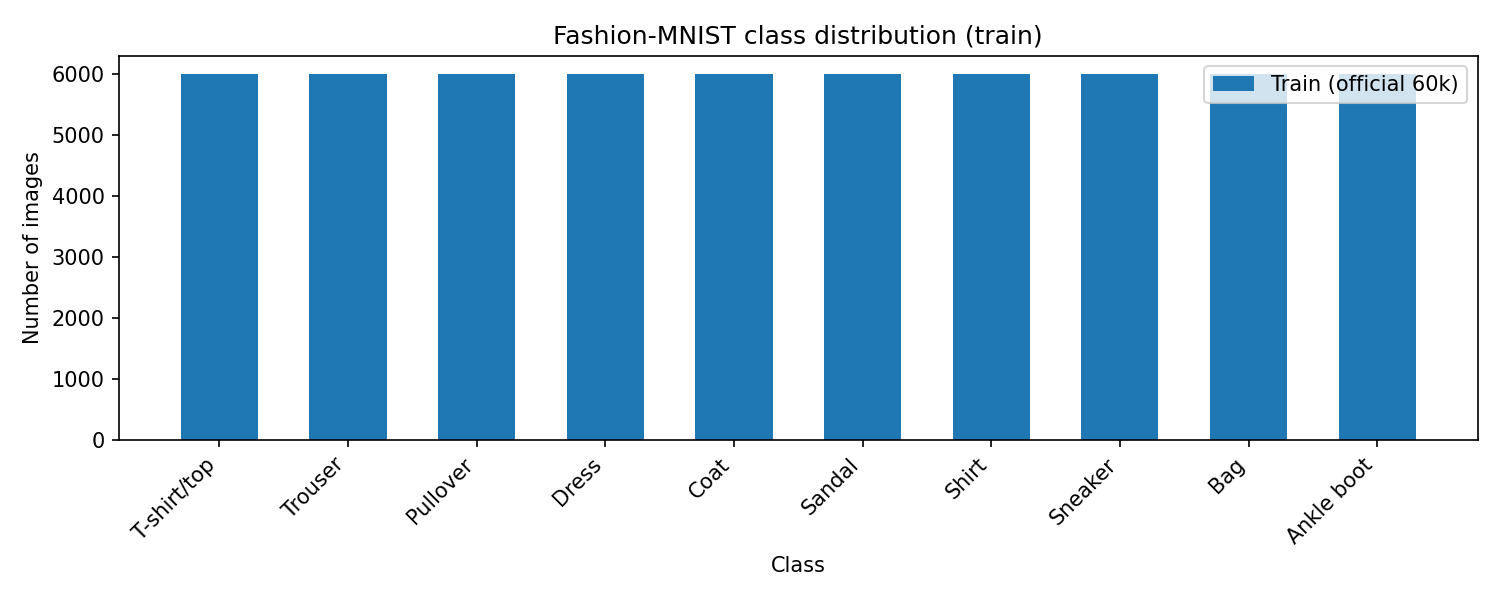
\includegraphics[width=\columnwidth]{figures/eda_class_distribution.png}
\caption{Number of images per class in the official training set (60{,}000 images).}
\label{fig:classdist}
\end{figure}

\begin{figure}[t]
\centering
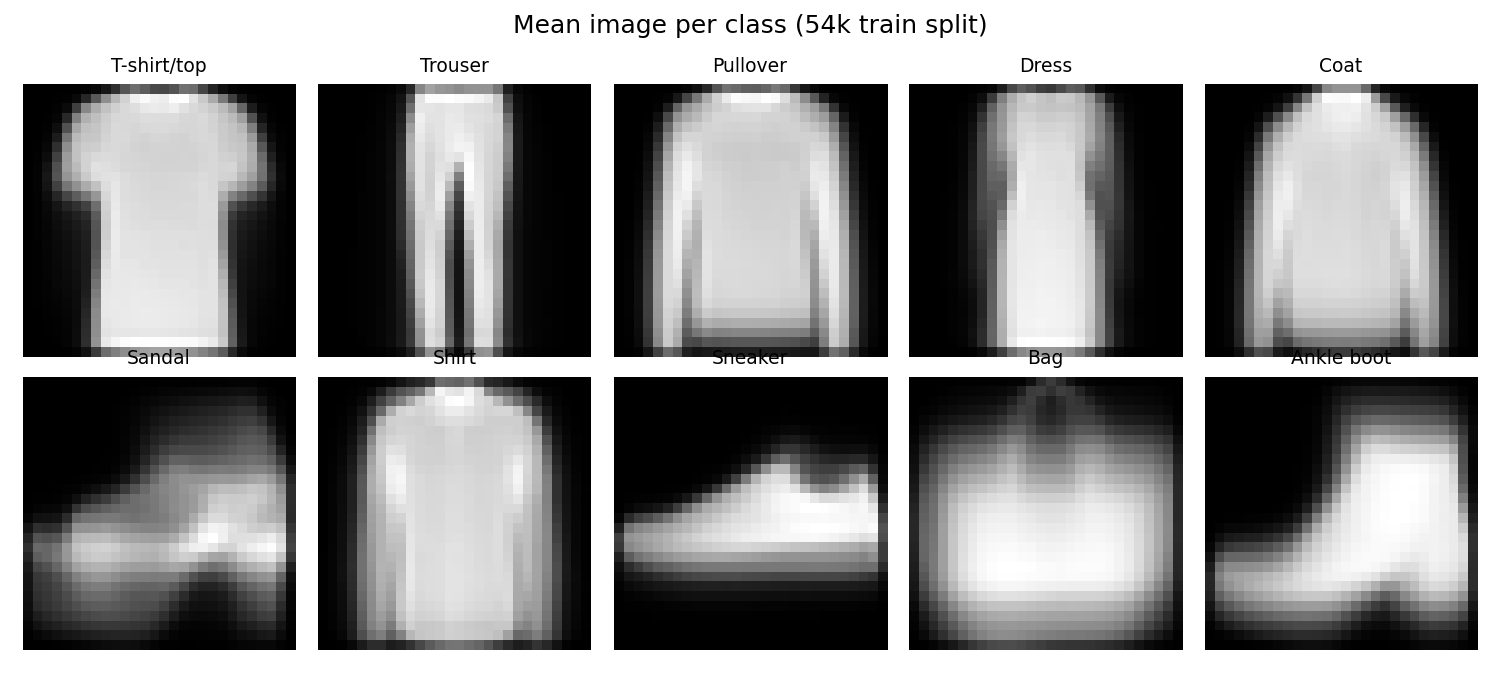
\includegraphics[width=\columnwidth]{figures/eda_mean_images.png}
\caption{Mean image of each class on the 54{,}000-image training split.}
\label{fig:means}
\end{figure}

\begin{figure}[t]
\centering
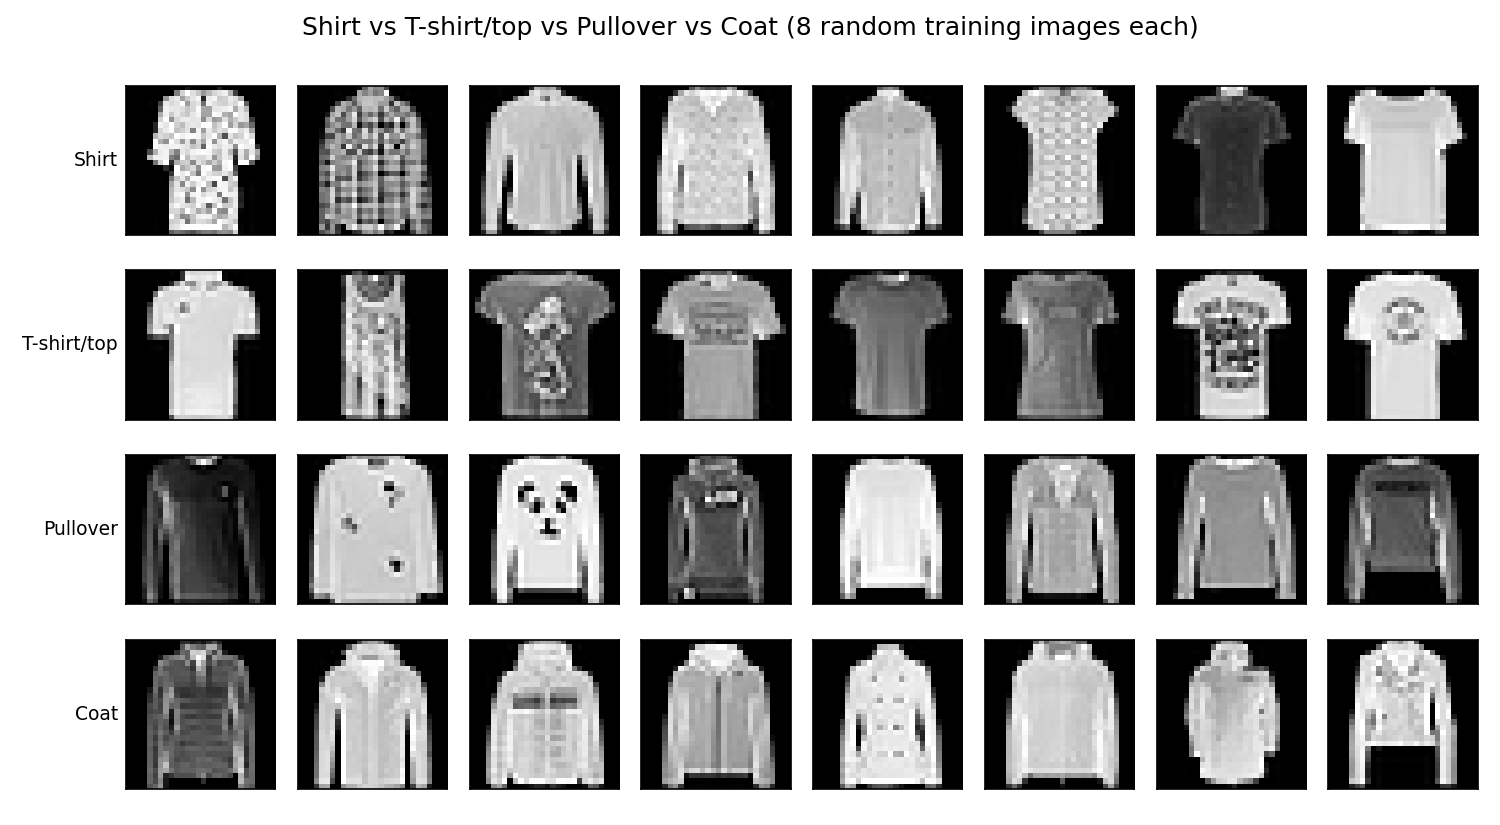
\includegraphics[width=\columnwidth]{figures/eda_confusable_panel.png}
\caption{Eight random training images each of Shirt, T-shirt/top, Pullover and Coat.}
\label{fig:panel}
\end{figure}

\begin{figure}[t]
\centering
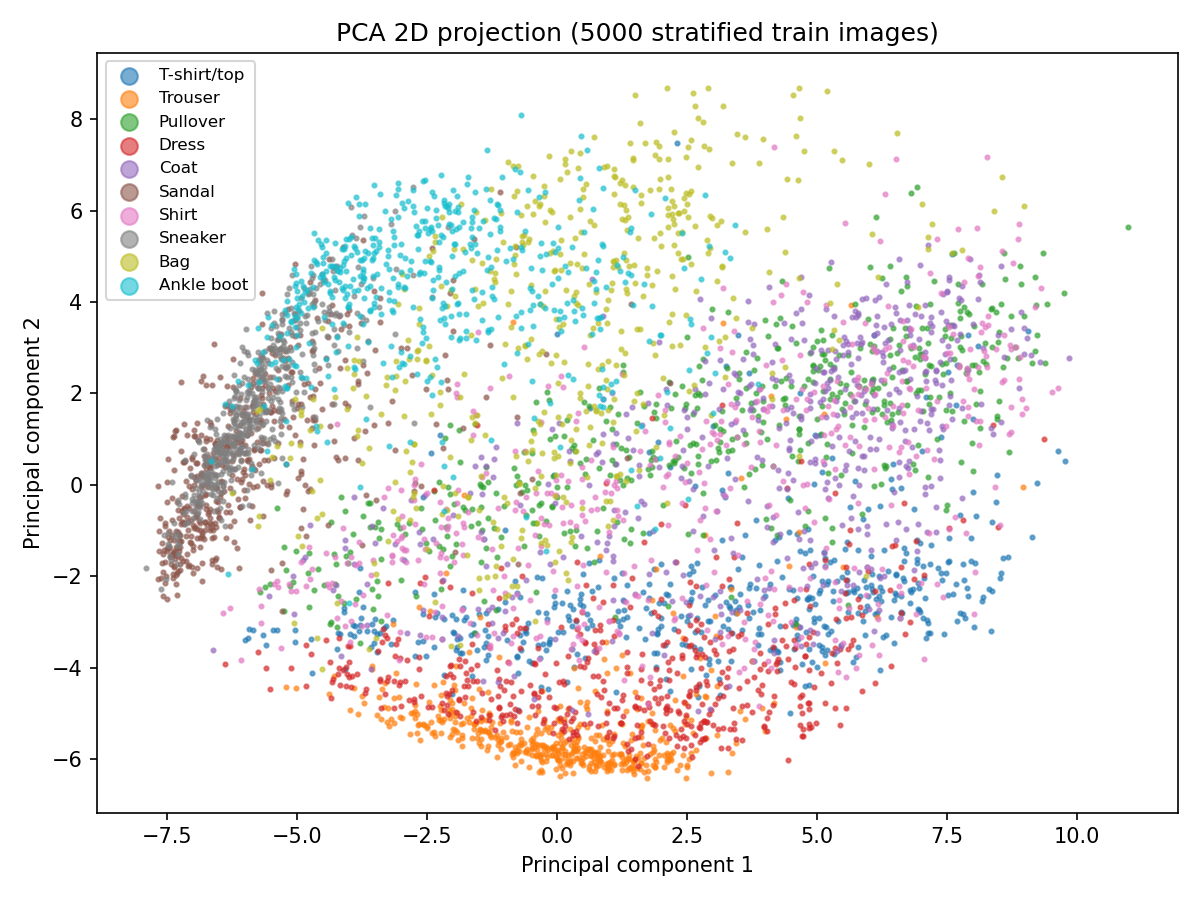
\includegraphics[width=\columnwidth]{figures/eda_pca_scatter.png}
\caption{PCA projection onto the first two components of 5{,}000 stratified training images, coloured by class. PCA was fitted on the training split only.}
\label{fig:pca}
\end{figure}

\begin{figure}[t]
\centering
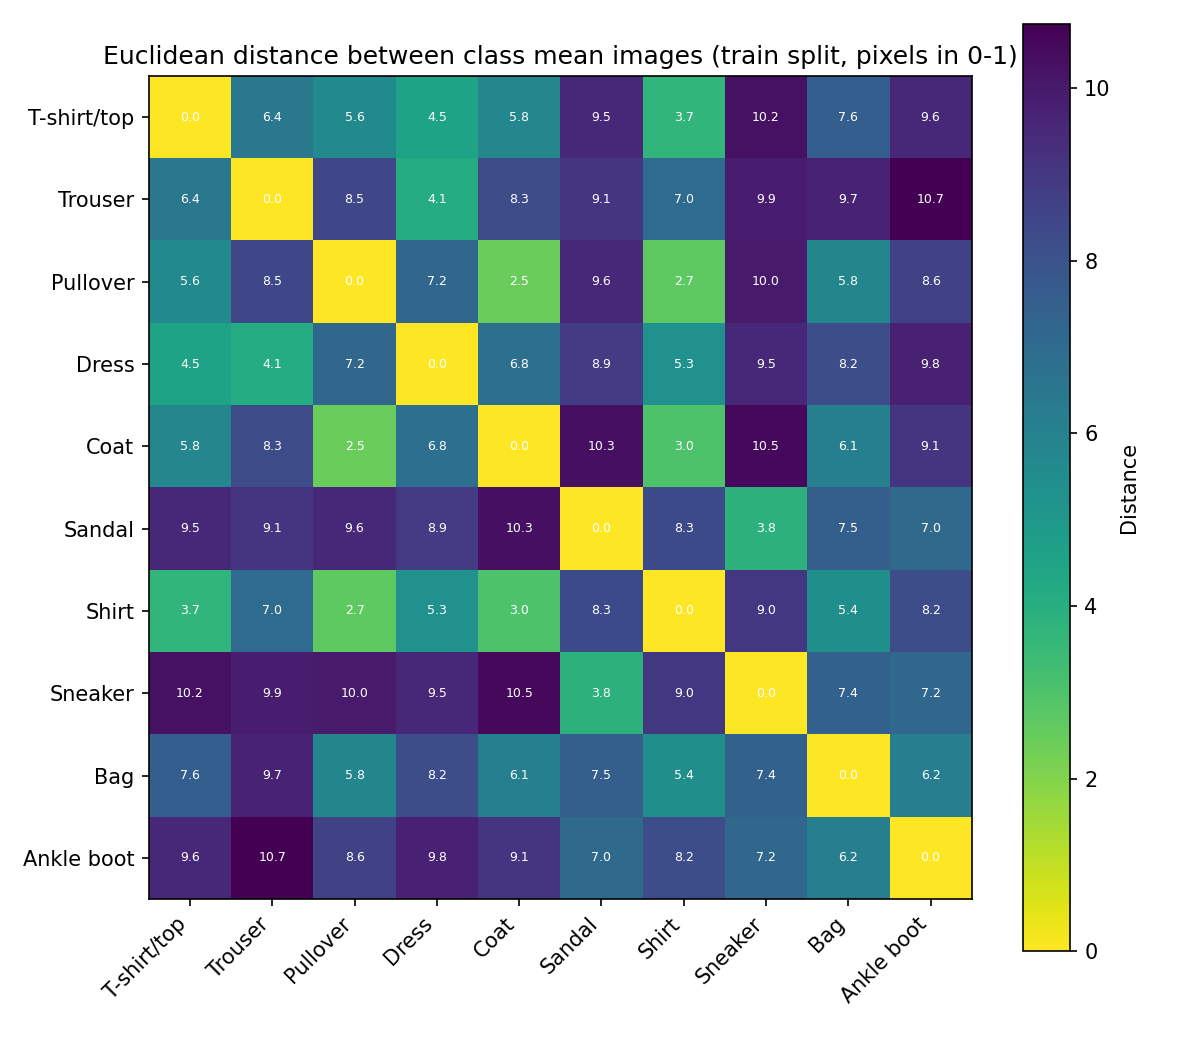
\includegraphics[width=\columnwidth]{figures/eda_centroid_heatmap.png}
\caption{Euclidean distance between class mean images on the training split (pixels scaled to 0--1).}
\label{fig:centroid}
\end{figure}


\section{Methodology and Preprocessing}
\label{sec:method}
We use the official split only. The 60{,}000 official training images are divided into a stratified
54{,}000-image training split and a 6{,}000-image validation split with seed 42; the 10{,}000 official test
images are used for evaluation only once, at the final test gate (Section~\ref{sec:protocol}); before the gate they are read only for loading and duplicate checks, and no test statistic enters any fitting or selection step. Nothing (scalers, mean and
standard deviation, or any other fitted preprocessing) is fitted on validation or test data. Pixel features are
scaled to $[0,1]$. Logistic regression and the SVM use a standardisation step inside the pipeline; $k$-NN and
random forest use no scaler; the CNN uses the mean and standard deviation of the training split. Final models are
trained on the 54{,}000-image training split only, with no refit on training plus validation.

\begin{table}[t]
\centering
\caption{Data splits used in all experiments.}
\label{tab:splits}
\begin{tabular}{lrl}
\toprule
Split & Images & Use \\
\midrule
Train & 54{,}000 & fitting \\
Validation & 6{,}000 & model selection \\
Test & 10{,}000 & final evaluation, once \\
\bottomrule
\end{tabular}
\end{table}

\section{Handcrafted Feature Engineering}
\label{sec:features}
We use two fixed representations. \emph{Flattened pixels} are the $28\times28$ image reshaped row by row into a
784-dimensional vector with values in $[0,1]$. They keep the absolute grey level at every location but treat each pixel
as an independent column: logistic regression, $k$-NN with Euclidean distance, the RBF-SVM and the random forest give
the same results if the columns of all images are permuted in the same way, so these models cannot use the fact that
two pixels are neighbours.

\emph{Histogram of oriented gradients} (HOG)~\cite{dalal2005histograms} describes local edge structure. We use the
implementation in scikit-image~\cite{vanderwalt2014scikit}: image gradients are computed per pixel; each cell of
$4\times4$ pixels collects a histogram of 9 unsigned orientation bins (0--180$^\circ$) weighted by gradient magnitude;
overlapping blocks of $2\times2$ cells, moved one cell at a time, are normalised with L2-Hys (L2 normalisation,
clipping at 0.2, renormalisation) and concatenated. For a $28\times28$ image, the selected $2\times2$-pixel cells give 14 cells per axis; with overlapping $2\times2$-cell blocks there are 13 blocks per axis. The resulting feature vector has length
\begin{equation}
13\cdot 13\cdot(2\cdot 2)\cdot 9 = 6084.
\end{equation}
which we verified against the library output. Block normalisation makes the descriptor less sensitive to local
contrast, but HOG discards absolute grey level.

\paragraph{HOG parameter study.}
Before any model comparison, the HOG parameters could change once, based on validation data only. Four
configurations (the baseline with $4\times4$-pixel cells, $7\times7$-pixel cells, $2\times2$-pixel cells, and 6 orientations) were compared with
logistic regression trained on a stratified 10{,}000-image subset of the training split and scored on the validation
split. The decision rule was fixed in advance: switch only if the validation macro-F1 exceeds the baseline by more than
0.010; otherwise keep the baseline. The study uses one model, one subset and one seed, so it is evidence for a choice
and not proof of the best descriptor. Outcome: the $2\times2$-pixel-cell configuration was selected. Its validation macro-F1 was 0.868348, compared with 0.836344 for the $4\times4$ baseline, an increase of 0.032004, exceeding the pre-set 0.010 threshold. The selected HOG vector has 6,084 features. The comparison used a stratified 10,000-image training subset and validation data only.

\paragraph{Leakage.}
HOG and flattening are fixed functions applied to each image independently; nothing is fitted, so computing them on
all splits creates no leakage. Features are cached on disk and keyed by their kind, split, image count and HOG
parameters. The only fitted preprocessing, the standardisation used by logistic regression and the SVM, sits inside the
model pipeline and is fitted on the training split.


\section{Classical Machine Learning Models}
\label{sec:classical}
We compare four classifiers on two representations (flattened pixels, 784 features; HOG, 6084 features),
giving eight experiments. All models are trained on the 54{,}000-image training split; hyperparameters
are chosen by validation macro-F1 on the 6{,}000-image validation split.

\subsection{Logistic Regression}
For $K=10$ classes, the multinomial model gives
\begin{equation}
p(y=k\mid \mathbf{x}) = \frac{\exp(\mathbf{w}_k^{\top}\mathbf{x}+b_k)}{\sum_{j=1}^{K}\exp(\mathbf{w}_j^{\top}\mathbf{x}+b_j)},
\end{equation}
trained by minimising the L2-regularised cross-entropy
\begin{equation}
\min_{W,\mathbf{b}}\ \tfrac12\lVert W\rVert_F^2 + C\sum_{i=1}^{N}-\log p(y_i\mid \mathbf{x}_i).
\end{equation}
Features are standardised using training-split statistics only.

\subsection{$k$-Nearest Neighbours}
Following Cover and Hart~\cite{cover1967nearest}, a query image is assigned the majority class among its $k$ nearest training images under Euclidean distance
$d(\mathbf{x},\mathbf{x}')=\lVert \mathbf{x}-\mathbf{x}'\rVert_2$. Small $k$ gives low bias and high variance.
Training stores the data; the cost is paid at prediction time. Features are not rescaled.

\subsection{Random Forest}
A random forest~\cite{breiman2001random} combines trees: each of 200 trees is grown on a bootstrap sample, and each split considers a random subset of features.
The forest predicts by averaging tree class probabilities. Splits are threshold tests on single features,
so the model is invariant to monotone feature rescaling.

\subsection{RBF Support Vector Machine}
The support vector machine~\cite{cortes1995support} uses the kernel $K(\mathbf{x},\mathbf{x}')=\exp(-\gamma\lVert \mathbf{x}-\mathbf{x}'\rVert^2)$ and the soft-margin problem is
\begin{equation}
\min_{\mathbf{w},b,\boldsymbol{\xi}}\ \tfrac12\lVert \mathbf{w}\rVert^2 + C\sum_i \xi_i
\quad \text{s.t. } y_i(\mathbf{w}^{\top}\phi(\mathbf{x}_i)+b)\ge 1-\xi_i,\ \xi_i\ge 0 .
\end{equation}
Multiclass prediction uses one-vs-one voting (45 binary classifiers for 10 classes).
Hyperparameters were tuned on a stratified 10{,}000-image subset (see limitations).

\subsection{Hyperparameter grids and runtime gate}
The grids searched on the validation split are in Table~\ref{tab:grids}; all other settings are library defaults
except those stated above (random forest: 200 trees; SVM: RBF kernel with $\gamma=$ ``scale''; logistic regression:
at most 500 iterations). The selected value is the one with the highest validation macro-F1, with validation accuracy
breaking ties. Before every final fit the fit time is estimated; a model whose estimate exceeds 30 minutes would be
fitted on a disclosed stratified subset, and the number of training images used is always reported. In the completed run, seven classical configurations used all 54,000 training images. The HOG RBF-SVM was runtime-gated to a stratified subset of 11,770 images because its estimated full fit exceeded the 30-minute limit. Final fit times ranged from 0.02 seconds for pixel k-NN to 393.61 seconds for HOG logistic regression. The pixel logistic-regression fit reached the configured 500-iteration limit with a convergence warning; its result is reported as run, not as proof of convergence.

\begin{table}[t]
\centering
\caption{Hyperparameter grids (validation macro-F1 selects the value).}
\label{tab:grids}
\footnotesize
\begin{tabular}{ll}
\toprule
Model & Grid \\
\midrule
Logistic regression & $C\in\{0.1,\,1.0\}$ \\
$k$-NN & $k\in\{3,\,5,\,7,\,11\}$ \\
Random forest & minimum leaf size $\in\{1,\,3\}$ \\
RBF-SVM & $C\in\{1,\,10\}$ \\
\bottomrule
\end{tabular}
\end{table}


\section{CNN Architecture and Training}
\label{sec:cnn}
The CNN has three convolution blocks followed by a two-layer classifier (Table~\ref{tab:cnn}).
Inputs are $28\times28$ grayscale images, scaled to $[0,1]$ and standardised with the mean and standard
deviation of the 54{,}000-image training split only. The network outputs ten raw logits; the softmax is
applied inside the loss and when probabilities are reported.

\begin{table}[t]
\centering
\caption{CNN layers and trainable parameters (the total is verified by code).}
\label{tab:cnn}
\footnotesize
\begin{tabular}{llrl}
\toprule
Layer & Output shape & Params & Calculation \\
\midrule
Conv $3{\times}3$, 1$\to$32, ReLU, MaxPool 2 & $32{\times}14{\times}14$ & 320 & $32(1\cdot 9+1)$ \\
Conv $3{\times}3$, 32$\to$64, ReLU, MaxPool 2 & $64{\times}7{\times}7$ & 18{,}496 & $64(32\cdot 9+1)$ \\
Conv $3{\times}3$, 64$\to$128, ReLU, MaxPool 2 & $128{\times}3{\times}3$ & 73{,}856 & $128(64\cdot 9+1)$ \\
Flatten, Dropout, Linear, ReLU & 128 & 147{,}584 & $1152\cdot128+128$ \\
Dropout, Linear & 10 & 1{,}290 & $128\cdot10+10$ \\
\midrule
Total & & 241{,}546 & \\
\bottomrule
\end{tabular}
\end{table}

Each convolution uses padding 1, so only pooling changes the spatial size; $7\to3$ uses floor division, so the last
row and column of the $7\times7$ map are ignored. Dropout~\cite{srivastava2014dropout} ($p=0.5$) is applied only in the classifier, which holds
most of the parameters.

\paragraph{Training.}
We minimise the cross-entropy loss with Adam~\cite{kingma2015adam} (learning rate $10^{-3}$, batch size 128,
at most 30 epochs). Mini-batches are shuffled with a seeded generator. After every epoch the validation loss and
accuracy are computed in evaluation mode (dropout off). Training stops when the validation loss has not improved for
5 consecutive epochs, and the weights of the best epoch are restored; the test images play no role in this
procedure. Training loss and accuracy in Fig.~\ref{fig:curves} are running averages over the mini-batches of
each epoch with dropout active, so they are pessimistic compared with an evaluation-mode pass. The learning rate,
batch size and dropout were not tuned. All results are from a single run with seed 42; run-to-run variation is not
measured. The recorded run lasted 29 epochs and restored the best checkpoint from epoch 24 (validation accuracy 0.9352, validation loss 0.1783). Training took 49.01 seconds on a Tesla T4 GPU. The final test accuracy was 0.9274 and macro-F1 was 0.9269.

\begin{figure}[t]
\centering
\figfile{cnn_learning_curves.png}{CNN learning curves}
\caption{CNN training and validation learning curves; the dashed line marks the epoch whose weights were kept.}
\label{fig:curves}
\end{figure}


\section{Experimental Protocol and Evaluation Metrics}
\label{sec:protocol}
Model selection uses the highest validation macro-F1, with validation accuracy breaking ties; the SVM is tuned
on a stratified 10{,}000-image subset of the training split. Before every final classical fit the fit time is
estimated, and if it exceeds the limit the model is fitted on a disclosed stratified subset; the number of
training images used is always reported. After selection the chosen configurations are written to a freeze file
and all nine models are evaluated on the test images exactly once. 

\paragraph{Metrics.}
Accuracy is the fraction of correctly classified images. For class $c$, $F1_c = 2TP_c/(2TP_c+FP_c+FN_c)$, and
macro-F1 is the unweighted mean of the ten $F1_c$ values, so every class counts equally. The test set has exactly
1{,}000 images per class, so macro-averaged recall equals accuracy; macro-F1 differs because it also depends on
precision. Confusion matrices have the true class in rows and the predicted class in columns.

\paragraph{Uncertainty and paired comparison.}
We report 95\% percentile bootstrap confidence intervals~\cite{efron1979bootstrap}: the 10{,}000 test images are
resampled with replacement 1000 times (seed 42). These intervals capture the sampling noise of this test set for one
trained model; they do not include the randomness of training. To compare the CNN with each classical model on the
same images we use McNemar's test~\cite{mcnemar1947note} on the paired correctness of the two models (exact binomial
test when there are fewer than 25 discordant pairs, otherwise a chi-square statistic with continuity correction), with a
Bonferroni correction for the eight comparisons. This test also ignores training variance~\cite{dietterich1998approximate}.

\paragraph{Inference cost.}
Timing uses the same 10{,}000 test images in a fixed order, and excludes model loading, training and plotting. For the
classical models we report ``predict only'' (precomputed features) and ``end-to-end'' (feature extraction from the raw
images, then prediction) separately, as the median of three repeats after an untimed warm-up call. For the CNN the inputs
are pre-normalised tensors, batch size 256, with three warm-up batches and the median of five repeats; the CPU is
mandatory and a GPU is used if available. The notebook records the library versions and the hardware it ran on
(\texttt{results/environment.json}); implementations are scikit-learn~\cite{pedregosa2011scikit},
PyTorch~\cite{paszke2019pytorch} and scikit-image~\cite{vanderwalt2014scikit}.

\section{Results and Comparative Analysis}
\label{sec:results}
% Owner: Rohan. Fill every cell from results/*.csv and results/*.json; never retype numbers by hand.
\IfFileExists{results_table.tex}{\begin{table*}[t]
\centering
\caption{Held-out test performance. Parentheses show 95\% percentile bootstrap confidence intervals from 1,000 resamples. The official test gate was run once.}
\label{tab:results}
\small
\begin{tabular}{llrcc}
\toprule
Model & Representation & $n_{\mathrm{train}}$ & Accuracy (95\% CI) & Macro-F1 (95\% CI) \\
\midrule
Logistic regression & pixels & 54,000 & 0.8411 (0.8338--0.8482) & 0.8403 (0.8336--0.8474) \\
k-NN & pixels & 54,000 & 0.8500 (0.8434--0.8567) & 0.8493 (0.8430--0.8559) \\
Random forest & pixels & 54,000 & 0.8756 (0.8693--0.8818) & 0.8741 (0.8682--0.8800) \\
RBF-SVM & pixels & 54,000 & 0.8953 (0.8887--0.9014) & 0.8951 (0.8889--0.9008) \\
Logistic regression & HOG & 54,000 & 0.8698 (0.8632--0.8766) & 0.8702 (0.8637--0.8764) \\
k-NN & HOG & 54,000 & 0.8653 (0.8583--0.8718) & 0.8621 (0.8555--0.8682) \\
Random forest & HOG & 54,000 & 0.8636 (0.8571--0.8703) & 0.8618 (0.8554--0.8682) \\
RBF-SVM & HOG & 11,770 & 0.8817 (0.8753--0.8879) & 0.8816 (0.8755--0.8877) \\
Small CNN & learned & 54,000 & 0.9274 (0.9219--0.9327) & 0.9269 (0.9214--0.9321) \\
\bottomrule
\end{tabular}
\end{table*}
}{%
\begin{table}[t]
\centering
\caption{Test results for the nine models (measured once at the test gate).}
\label{tab:results}
\begin{tabular}{llrr}
\toprule
Model & Representation & Accuracy & Macro-F1 \\
\midrule
Logistic regression & pixels & \TBD & \TBD \\
$k$-NN & pixels & \TBD & \TBD \\
Random forest & pixels & \TBD & \TBD \\
RBF-SVM & pixels & \TBD & \TBD \\
Logistic regression & HOG & \TBD & \TBD \\
$k$-NN & HOG & \TBD & \TBD \\
Random forest & HOG & \TBD & \TBD \\
RBF-SVM & HOG & \TBD & \TBD \\
Small CNN & learned & \TBD & \TBD \\
\bottomrule
\end{tabular}
\end{table}

}

\IfFileExists{inference_table.tex}{\begin{table*}[t]
\centering
\caption{Inference timing on 10,000 test images. Classical values are single timed passes after an untimed warm-up; treat as preliminary. Predict-only uses precomputed features, while end-to-end includes feature extraction. CNN CPU/GPU timing uses pre-normalised tensors and is not directly comparable to classical end-to-end timing.}
\label{tab:inference}
\small
\begin{tabular}{llrrrr}
\toprule
Model & Representation & Predict-only CPU (ms/img) & End-to-end CPU (ms/img) & CNN GPU (ms/img) & Fit time (s) \\
\midrule
Logistic regression & pixels & 0.008830 & 0.010633 & -- & 131.48 \\
k-NN & pixels & 2.255952 & 2.120674 & -- & 0.02 \\
Random forest & pixels & 0.056275 & 0.048987 & -- & 125.09 \\
RBF-SVM & pixels & 14.804295 & 14.560057 & -- & 267.66 \\
Logistic regression & HOG & 0.056755 & 3.302105 & -- & 393.61 \\
k-NN & HOG & 15.137228 & 18.482470 & -- & 0.12 \\
Random forest & HOG & 0.082839 & 3.329037 & -- & 348.48 \\
RBF-SVM & HOG & 48.426658 & 51.899920 & -- & 322.48 \\
Small CNN & learned & 0.440153 & not measured & 0.011625 & 49.01 \\
\bottomrule
\end{tabular}
\end{table*}
}{%
\begin{table}[t]
\centering
\caption{Inference time per image and parameter counts. \TBD}
\label{tab:inference}
\begin{tabular}{lrr}
\toprule
Model & ms/img (CPU) & Parameters \\
\midrule
\TBD & \TBD & \TBD \\
\bottomrule
\end{tabular}
\end{table}

}

\begin{figure}[t]
\centering
\figfile{model_comparison.png}{TBD: model comparison plot}
\caption{Accuracy and macro-F1 of the nine models on the test set with 95\% bootstrap confidence intervals.}
\label{fig:comparison}
\end{figure}

\section{Confusion Matrices and Error Analysis}
\label{sec:errors}
% Owner: Rohan (LaTeX-ready section to be merged).
\TBD

\begin{figure}[t]
\centering
\figfile{cm_cnn.png}{TBD: confusion matrix}
\caption{Row-normalised confusion matrix of the CNN on the test set (rows: true class).}
\label{fig:confusion}
\end{figure}

\begin{figure}[t]
\centering
\figfile{per_class_recall.png}{TBD: per-class recall heatmap}
\caption{Per-class recall of the nine models on the test set.}
\label{fig:recall}
\end{figure}

\section{Discussion, Limitations and Future Improvements}
\label{sec:discussion}
\TBD{} (after results.)

\section{Conclusion}
\label{sec:conclusion}
\TBD{} (after results.)

\section*{Acknowledgment}
\TBD

\bibliographystyle{IEEEtran}
\bibliography{references}

\end{document}
